\documentclass[11pt]{article}
\usepackage[a4paper, total={6in, 8in}]{geometry}
\usepackage{graphicx} 
\usepackage{amsmath}
\usepackage{listings}
\usepackage{hyperref}
\usepackage{listings}
\usepackage{algorithm}
\usepackage{algorithmic}
\usepackage{booktabs}
\usepackage{longtable}
\usepackage{titling}
\usepackage{xcolor}
\usepackage{colortbl}
\usepackage[backend=biber,style=numeric]{biblatex}

\DeclareFieldFormat[book]{chapter}{#1}
\renewbibmacro*{bbx:chapter+editor+title}{%
  \printfield{chapter}%
  \setunit{\addspace}%
  \printnames{editor}%
  \newunit
  \printfield{title}%
}

\addbibresource{references.bib}

% Packages for formatting
\usepackage{graphicx}
\usepackage{lipsum} % For dummy text (remove this in actual document)
\usepackage{geometry}
\geometry{a4paper, margin=1in}

% Customization for title page
\begin{document}

\begin{titlepage}
    \centering
    {\Huge \textbf{Deep Learning for Video Action Recognition: Implementation and Evaluation of Models on the UCF101 Dataset} \par}
    \vspace{2cm}
    
    {\Large Master Degree in Artificial Intelligence \par}
    \vspace{0.5cm}
    
    {\Large Course: Deep Learning \par}
    \vspace{0.5cm}
    
    {\Large Academic Year: 2025 - 2026 \par}
    \vfill
    
    \textbf{Author:} \\
    Fidanza Riccardo - VR516130\\
    \vspace{1cm}

    
\includegraphics[width=0.3\textwidth]{images/logo.png}
    \vspace{1cm}
    
    {\Large University of Verona \par}
    \vspace{0.5cm}
    
    {\Large June, 2026 \par}
\end{titlepage}


\begin{abstract}
\noindent Human Action Recognition (HAR) remains a pivotal challenge in computer vision due to the complex interplay between spatial context and temporal dynamics. This study presents a systematic comparative analysis of different architectural paradigms for action classification on the UCF101 dataset, tracking the technological evolution from simple spatial feature aggregation to state-of-the-art attention-based systems. We implement and evaluate three distinct models: a baseline 2D CNN (ResNet), a recurrent sequential model (ResNet18-LSTM, ResNet18-BiLSTM), and a Video Masked Autoencoder (VideoMAE) based on the Vision Transformer (ViT) architecture. Our results demonstrate a clear performance hierarchy: while the BiLSTM model achieves a solid test accuracy of 78.14\%, effectively capturing mid-range temporal dependencies, the VideoMAE architecture establishes the study’s benchmark with a peak accuracy of 82.76\%. Despite observing a significant generalization gap due to rapid training saturation on a medium-scale dataset, the Transformer-based approach confirms the superiority of global self-attention over recurrent hidden states. Furthermore, we provide a critical discussion on the discrepancy between our single-view inference results and published state-of-the-art benchmarks (96.1\%), identifying multi-view evaluation and aggressive data augmentation as the primary drivers for peak performance. This work validates the transition toward attention-centric modeling as the most effective path for robust and efficient spatiotemporal representation learning.
\end{abstract}

\newpage 
\tableofcontents

\section{Introduction}


\subsection{Motivation and Objectives}
The fundamental challenge in Human Action Recognition (HAR) lies in the effective integration of spatial and temporal information. While deep learning has largely mastered static image classification, video understanding remains complex due to the necessity of interpreting motion over time. This project is motivated by the need to systematically evaluate how different architectural paradigms from simple spatial extractors to complex attention-based models—handle these spatiotemporal demands using the UCF101 benchmark.\\
The rationale behind our incremental approach is to map the transition from "scene recognition" to "true action understanding" through three distinct phases:
\begin{enumerate}
    \item Spatial Baseline: first examine models restricted to spatial features. This stage establishes a performance floor, identifying which actions can be guessed simply by recognizing the environment or objects present in the frames.
    \item Recurrent Modeling: The goal is to quantify the "value of time" by measuring improvements in classes where the chronological order of movement is the primary identifier.
    \item Attention Mechanisms: Finally, Transformer-based architectures were implemented to evaluate if attention can capture dependencies more effectively than the hidden states of recurrent networks.
\end{enumerate}
Ultimately, this study aims to provide a granular understanding of model behavior. Rather than focusing solely on overall accuracy, I perform a class-level analysis to identify the best and worst performing categories for each model. This allows us to observe which actions are "temporally sensitive" and which are "spatially dominated," providing clear insight into the strengths and limitations of each technological paradigm.


\subsection{State Of The Art}
The evolution of Action Recognition on the UCF101 dataset \cite{soomro2012ucf101} reflects the broader history of computer vision, moving from handcrafted descriptors to deep spatiotemporal architectures.\\
Table \ref{tab:sota_benchmarks} summarizes the Top-1 accuracy of milestone models on the UCF101 dataset. It is important to note that, for the purpose of this study, I report benchmarks referring exclusively to models utilizing \textbf{RGB input only}.\\
This focus is motivated by the significant computational overhead and storage requirements associated with the pre-computation of Optical Flow.

\begin{table}[h]
\centering
\begin{tabular}{lcl}
\toprule
\textbf{Paradigm} & \textbf{Accuracy (\%)} & \textbf{Reference Model} \\
\midrule
Recurrent (LRCN RGB) & 71.1\% & CNN+LSTM \cite{Donahue2015} \\
TSN (RGB only) & 86.4\% & Temporal Segment Networks \cite{Wang2016} \\
\textbf{Transformer} & \textbf{96.1\%} & \textbf{VideoMAE (Base)} \cite{Tong2022} \\
\bottomrule
\end{tabular}
\caption{Benchmark performance of different architectural paradigms on the UCF101 dataset (Split-1).}
\label{tab:sota_benchmarks}
\end{table}


\subsection{Objectives}

The primary objective of this study is to perform a systematic comparative analysis of different neural architectures for Human Action Recognition (HAR), tracking the technological evolution from simple spatial feature aggregation to state-of-the-art attention-based systems. The aim is to quantify the impact of temporal modeling on classification accuracy and identify the specific challenges associated with each paradigm. Specifically, the project pursues the following goals:

\begin{itemize}
    \item \textbf{Incremental Architectural Evaluation:} Build and train three distinct categories of models to observe the "performance gain" brought by increasingly complex temporal reasoning:
    \begin{enumerate}
        \item \textit{Bag of Frames:} To establish a performance floor and measure how much information can be extracted solely from static visual context.
        \item \textit{Recurrent Architectures} To evaluate the benefit of sequential modeling and hidden state memory in capturing the chronological order of actions.
        \item \textit{Vision Transformers:} To assess the effectiveness of global self-attention and masked autoencoding in learning high-level spatiotemporal representations.
    \end{enumerate}
    
    \item \textbf{Benchmarking Against State of the Art:} A key goal is to compare our experimental results with the established SOTA performance on the UCF101 dataset. This comparison allows us to validate our implementation and understand how modern pre-training techniques (such as those used in VideoMAE) bridge the gap between theoretical potential and practical accuracy on smaller datasets.
    
    \item \textbf{Qualitative and Class-Level Analysis:} Beyond overall accuracy, this study intends to investigate \textit{where} and \textit{why} specific architectures fail. By performing a per-class analysis, the aim is to determine which actions are "temporally sensitive" (requiring sequence knowledge) and which are "spatially dominated" (identifiable via single frames), thereby revealing the strengths and limitations of each technological paradigm.
\end{itemize}
\section{Methodology}


\subsection{Introduction to UCF101 Dataset}
The \textbf{UCF101} dataset \cite{soomro2012ucf101} serves as a fundamental benchmark for action recognition research in computer vision. It provides a diverse collection of \textbf{13,320 video clips} curated from YouTube, encompassing a wide array of human activities across \textbf{101 distinct action classes} (showned in Figure~\ref{fig:ucf101}). These classes range from fine-grained daily tasks, such as \textit{Brushing Teeth} or \textit{Applying Makeup}, to complex athletic maneuvers and musical performances.\\\\
The 101 categories are taxonomically organized into five primary types based on the nature of the movement and the entities involved:
\begin{itemize}
    \item \textbf{Human-Object Interaction:} Actions involving tools or equipment (e.g., Knitting, Hammering).
    \item \textbf{Body-Motion Only:} Purely physical movements without external objects (e.g., Baby Crawling, Jumping Jacks).
    \item \textbf{Human-Human Interaction:} Actions requiring multiple participants (e.g., Salsa Spin, Fencing).
    \item \textbf{Playing Musical Instruments:} Highly rhythmic and localized movements (e.g., Playing Cello, Playing Flute).
    \item \textbf{Sports:} Dynamic actions performed in specific athletic environments (e.g., Archery, Basketball Dunk).
\end{itemize}
\noindent
A defining structural feature of UCF101 is its hierarchical organization. Within each category, videos are partitioned into \textbf{25 distinct groups}, each containing \textbf{4 to 7 clips}. Videos belonging to the same group typically share significant contextual features, such as similar backgrounds, consistent viewpoints, and common subjects \cite{soomro2012ucf101}.

\begin{figure}[h]
    \centering
    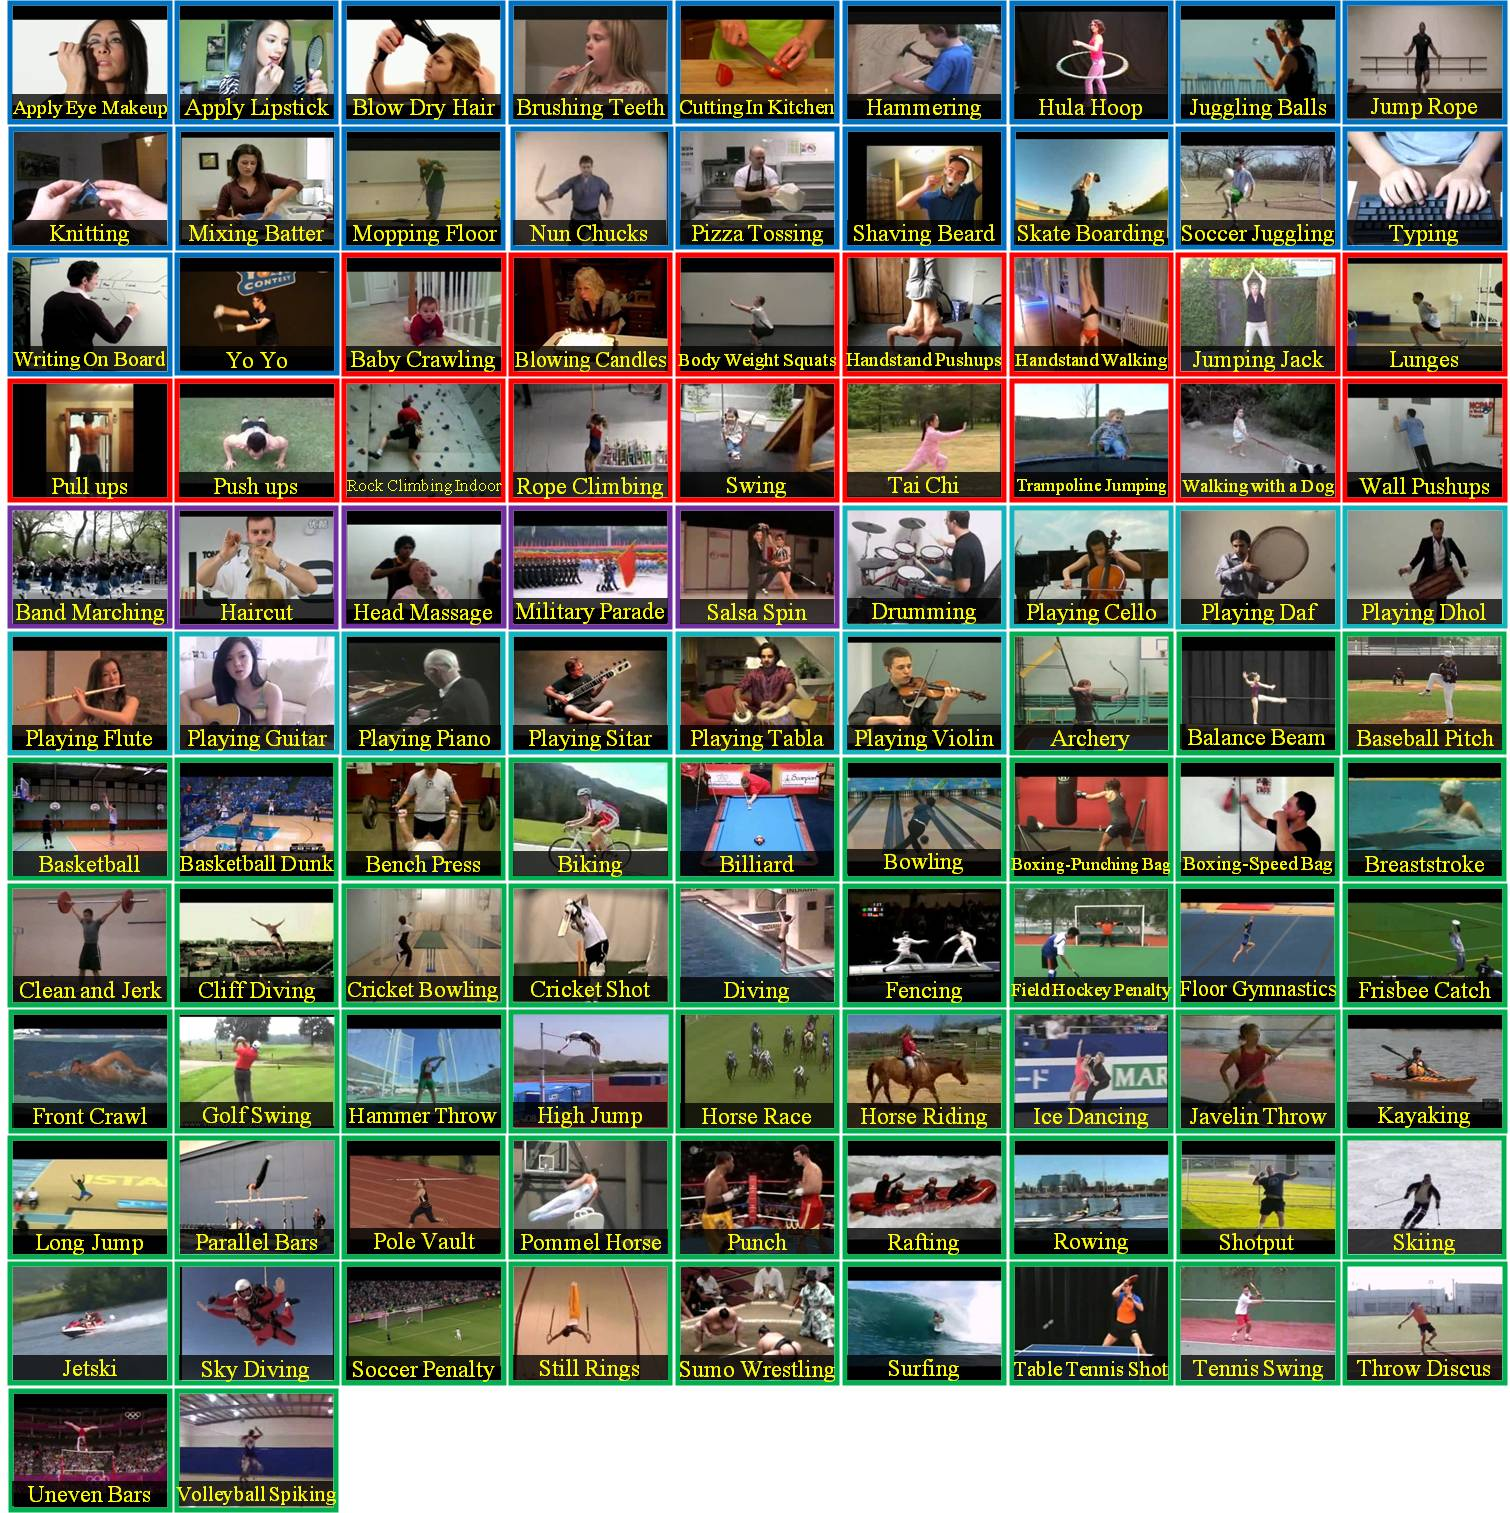
\includegraphics[width=0.5\textwidth]{images/classes.png}
    \caption{A representative frame for each action class in the UCF101 dataset. \cite{ucf101_website}.}
    \label{fig:ucf101}
\end{figure}


\subsection{Class Distribution Analysis}
Figure~\ref{fig:ucf101_cd} presents the distribution of video samples across the 101 action classes of the UCF101 dataset. The bar chart highlights a moderate degree of class imbalance: the most frequent class, \textit{Punch}, contains 121 samples, while the least represented class, \textit{TaiChi}, includes 72 samples. On average, each class is represented by approximately 94.4 video samples. Despite the non-uniform distribution, the ratio between the majority and minority classes remains below 2:1, indicating that the imbalance is relatively mild.\\
From a training perspective, this level of imbalance does not warrant the use of aggressive compensation techniques such as synthetic oversampling (e.g., SMOTE) or class-weighted loss functions. Instead, random shuffling is employed within the \texttt{DataLoader} to ensure that each mini-batch contains a stochastic mixture of action classes. This strategy reduces the risk of the model developing a bias toward more frequent actions during the gradient descent optimization process, while preserving the original data distribution.

\begin{figure}[h]
    \centering
    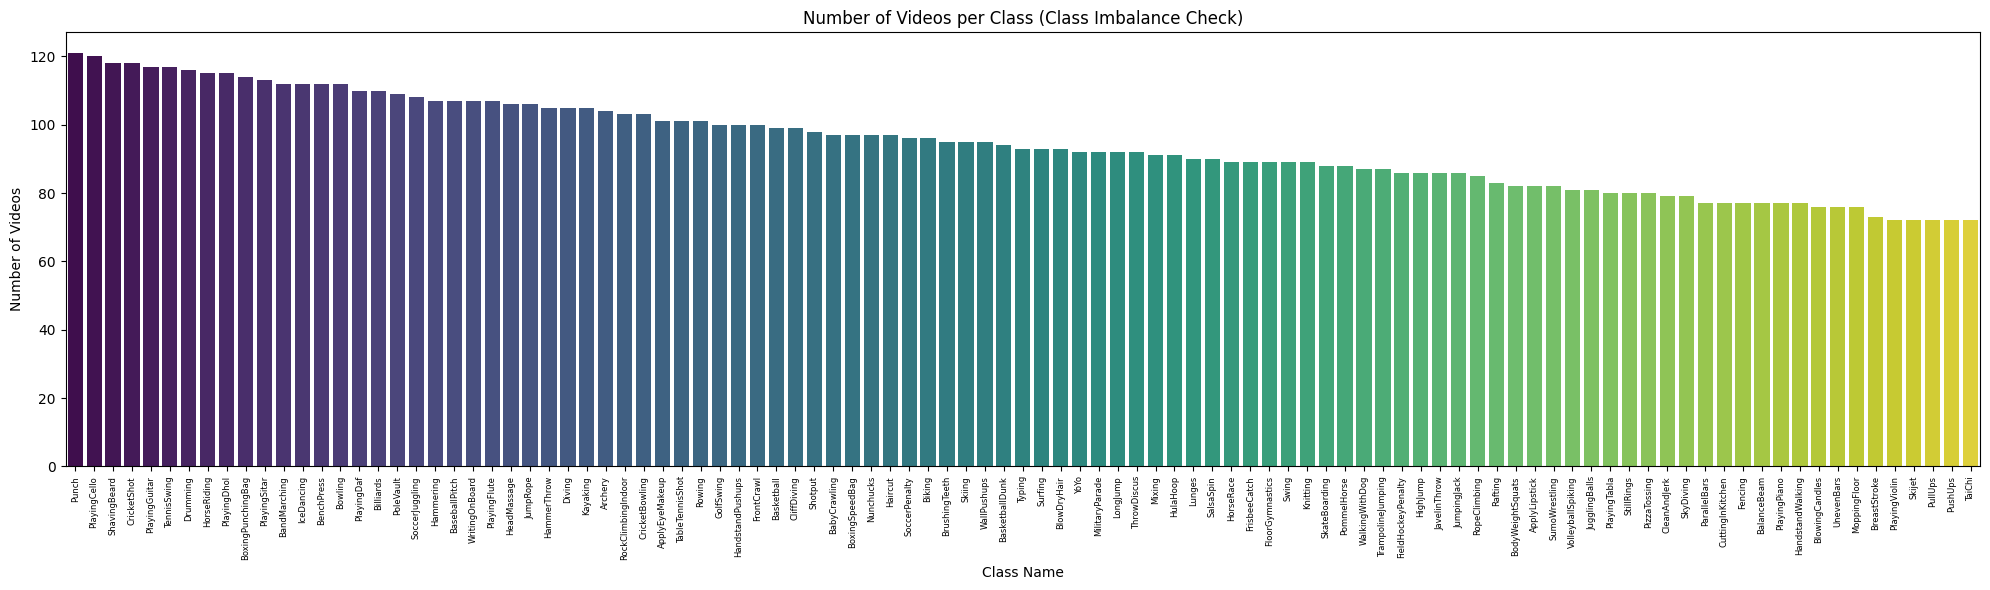
\includegraphics[width=1\textwidth]{images/CD.png}
    \caption{Class Distribution in UCF101 Dataset.}
    \label{fig:ucf101_cd}
\end{figure}

\subsection{Data Splitting and Integrity}
The division of the dataset follows a rigorous protocol to ensure the reliability of the results. While the training and test sets are provided directly by the original UCF101 creators \cite{soomro2012ucf101}, the validation set was extracted from the training partition using a \textbf{group-wise splitting strategy}.
This approach is fundamental to prevent \textbf{data leakage}: since videos in the same group often share the same subject, background, and camera viewpoint, a random split would allow the model to "memorize" specific environments. By isolating groups, the model is forced to generalize to unseen subjects and settings. Finally, an integrity check was performed post-split, confirming zero overlapping samples between the training, validation, and test sets, thus guaranteeing an honest assessment of the model's performance.

\subsection{Data Preprocessing and Pipeline}
To process the video data efficiently while preserving spatio-temporal information, the following preprocessing steps were implemented.

\subsubsection{I/O Optimization}
To mitigate the I/O bottleneck—a common challenge when handling thousands of video files—all extracted frames were converted and stored in \textbf{JPEG format}. This optimization significantly reduced disk read times during the training phase, allowing for a higher throughput of samples per second and ensuring that the GPU remains the primary computational bottleneck rather than the storage subsystem.

\subsubsection{Data Augmentation and Spatial Transformation}
To enhance the model's ability to generalize and to mitigate the spatial memorization often observed in high-capacity architectures, a dual-stage transformation pipeline was implemented:
\begin{itemize}
    \item \textbf{Training Augmentation:} During the training phase, \textbf{Random Horizontal Flips} ($p=0.5$) and \textbf{Color Jittering} (adjusting brightness and contrast by $10\%$) were applied. 
    \item \textbf{Standardized Preprocessing:} All frames across all sets were resized to a spatial resolution of $224 \times 224$ pixels. A standard normalization using mean $\mu = [0.485, 0.456, 0.406]$ and standard deviation $\sigma = [0.229, 0.224, 0.225]$, derived from the ImageNet dataset, was applied to align the input distribution with the pre-trained ResNet18 feature space.
\end{itemize}

\subsubsection{Temporal Sampling}
Video was reduced from its native length to a fixed temporal depth of $T=16$ frames. This represents significant a compression. The reasoning behind this choice is twofold:
\begin{enumerate}
    \item \textbf{High Temporal Redundancy:} Adjacent frames in video data are highly correlated and often contain minimal distinct semantic information. Processing every frame would lead to computational inefficiency and potential overfitting without a proportional gain in feature quality.
    \item \textbf{Global Uniform Sampling:} Rather than simple truncation (taking only the first few seconds), the pipeline employs a uniform sampling function. By extracting frames at equidistant intervals across the \textit{entire duration} of the clip, the model captures the full temporal evolution of the action, including the \textbf{onset, nucleus, and offset} phases.
\end{enumerate}
\noindent
This strategy ensures that the resulting tensor, with dimensions $(Batch \times 3 \times 16 \times 224 \times 224)$, remains compatible with GPU memory constraints while preserving the global context of the video sequence.

\subsection{Models}
Several models were implemented, ranging from a custom baseline to state-of-the-art attention-based architectures.

\subsubsection{Custom CNN with temporal mean pooling}
The initial phase of the study involves the design and implementation of a lightweight, shallow Convolutional Neural Network (CNN). This model serves as the experimental baseline, providing a performance floor against more sophisticated architectures.

\subsubsection*{Architectural Design}

The model in Figure~\ref{fig:cnn_custom} is composed of four sequential convolutional blocks. Each block follows a modular design: a 2D Convolutional layer with a $3 \times 3$ kernel, followed by \texttt{Batch Normalization} (BN) to stabilize training, a \texttt{ReLU} activation function, and a \texttt{MaxPool} layer for spatial downsampling.
The spatial resolution of the input frames evolves as follows:
\[
(3 \times 224 \times 224) \xrightarrow{\text{Block 1}} (32 \times 112 \times 112) \xrightarrow{\text{Block 2}} (64 \times 56 \times 56) \xrightarrow{\text{Block 3}} (128 \times 28 \times 28) \xrightarrow{\text{Block 4}} (256 \times 14 \times 14)
\]
A critical design choice is the inclusion of an \textbf{Global Average Pooling} (GAP) layer before the classification head. Instead of a standard flattening of the $256 \times 14 \times 14$ tensor—which would result in a massive fully connected layer ($50,176$ neurons). The GAP layer collapses the spatial dimensions into a $1 \times 1$ representation.

\begin{figure}[h]
    \centering
    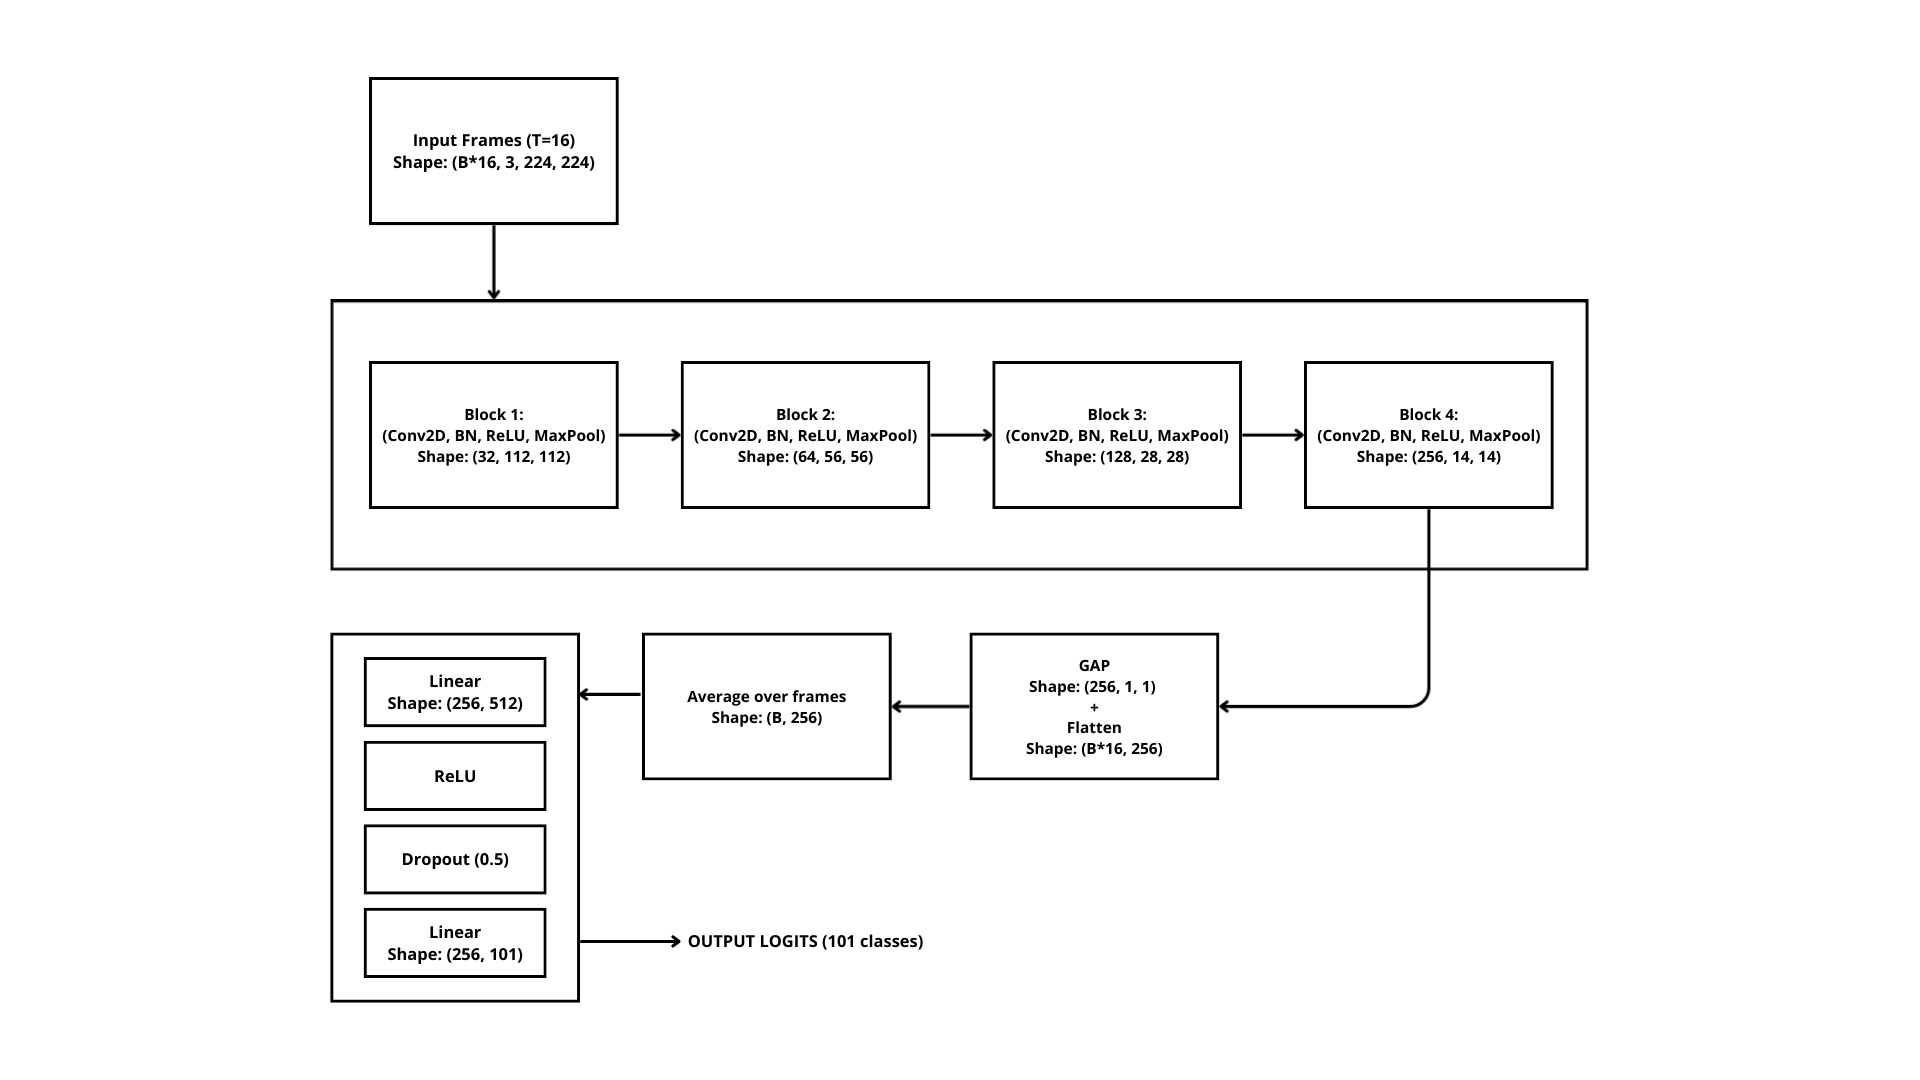
\includegraphics[width=1\textwidth]{images/CNN custom.png}
    \caption{Custom CNN Architecture.}
    \label{fig:cnn_custom}
\end{figure}
\noindent
After the GAP layer the model performs a \textbf{temporal mean pooling} across the sequence:$$ \mathbf{x}_{video} = \frac{1}{T} \sum_{t=1}^{T} \mathbf{x}_t $$
This aggregated vector $\mathbf{x}_{video}$ is then passed to the classification head. This "Bag-of-Frames" approach allows the model to capture the global visual context of the clip, although it remains invariant to the specific chronological order of the actions.


\subsubsection{ResNet18 Backbone with mean temporal pooling}

To overcome the structural limitations and the lack of representational depth of the custom baseline, we transition to a significantly more robust architecture based on ResNet18. This model is architecturally optimized for large-scale image recognition and is far better suited for the high-dimensional complexity of the UCF101 dataset. The primary advantages of this approach include the increased depth of the network, its ability to extract features, and the strategic use of \textbf{Transfer Learning} via weights pre-trained on the ImageNet-1K dataset.

\subsubsection*{Architectural Design}

The architecture of the proposed model, is built upon a modular design that balances feature reuse with specialized \textbf{fine-tuning}.
\begin{enumerate} 
    \item \textbf{Feature Extraction Backbone}: The model adopts a \textbf{ResNet18} architecture as its core feature extractor. 
    \item \textbf{Selective Layer Freezing}: To preserve the general-purpose visual features (such as edges and basic textures) while reducing the number of trainable parameters, a selective freezing strategy is applied. The initial convolutional layer (\texttt{conv1}), the first batch normalization layer (\texttt{bn1}), and the first two residual blocks (\texttt{layer1}, \texttt{layer2}) are frozen. Training is focused exclusively on the deeper layers which are responsible for capturing more abstract and task-specific semantic information.
    \item \textbf{Robust Classification Head}: The original fully connected layer of the ResNet is replaced with a custom module that incorporates a \textbf{Dropout} layer with a probability of $0.5$ that acts as a critical regularizer, followed by a final \textbf{Linear} layer mapping to the 101 classes of UCF101. 
    \item \textbf{Spatiotemporal Processing Pipeline}: The temporal dimension is aggregated via temporal mean pooling, keeping the model invariant to the chronological order of the sequence. 
\end{enumerate}

\subsubsection{ResNet18 + LSTM}
This architecture builds upon the ResNet18 backbone described previously but introduces an LSTM to capture the temporal evolution of the actions by processing the frames as a chronological sequence.

\subsubsection*{Architectural Design}

\begin{enumerate} 
    \item \textbf{Feature Extraction Backbone}: The ResNet18 architecture is employed as a spatial feature extractor, specifically fine-tuned on the UCF101 dataset.
    \item \textbf{Regularization}: a \textbf{Spatial Dropout} is applied immediately after the backbone to regularize the transition to the temporal module and mitigate overfitting.
    \item \textbf{LSTM Module}: A 2-layer \textbf{Unidirectional LSTM} with a hidden size of 1024 is utilized. It processes the sequence of 16 frames to model long-term temporal dependencies.
    \item \textbf{Temporal Aggregation}: The hidden states across the entire sequence are aggregated via \textbf{temporal mean pooling}:
    \[ \mathbf{h}_{pooled} = \frac{1}{T} \sum_{t=1}^{T} \mathbf{h}_t \]
    \noindent
    This ensures the final representation accounts for the whole sequence rather than just the last frame.
    \item \textbf{Classification Head}: A sequential MLP (Linear 1024 $\to$ 512, ReLU, Dropout 0.5, Linear $\to$ 101) for the final class prediction.
\end{enumerate}

\subsubsection{ResNet18 + BiLSTM}

This architecture upgrades the temporal module to a \textbf{Bidirectional LSTM (BiLSTM)}, allowing the network to capture dependencies from both past and future frame contexts simultaneously.

\begin{enumerate} 
    \item \textbf{Feature Extractor}: ResNet18 backbone (ImageNet pre-trained) for frame-level extraction, with full fine-tuning of all parameters enabled.
    \item \textbf{Regularization}: a \textbf{Spatial Dropout} is applied to the feature sequence to prevent overfitting.
    \item \textbf{BiLSTM Module}: a 2-layer Bidirectional LSTM with a hidden size of 512. The bidirectional configuration doubles the output dimensionality to 1024 by concatenating forward and backward hidden states.
    \item \textbf{Temporal Aggregation}: Global average pooling (mean) is performed across the temporal dimension to aggregate the BiLSTM outputs.
    \item \textbf{Classification Head}: A sequential MLP (Linear 1024 $\to$ 512, ReLU, Dropout 0.5, Linear $\to$ 101) for the final prediction.
\end{enumerate}

\subsubsection{Transformer-based Model: VideoMAE}

The VideoMAE (Video Masked Autoencoder) architecture represents a shift toward self-supervised, attention-based spatiotemporal modeling. VideoMAE utilizes a Vision Transformer (ViT) backbone to capture global dependencies across the entire video volume \cite{Tong2022}. 

\subsubsection*{Architectural Design}
The architecture follows the standard Vision Transformer (ViT) framework, adapted for video through 3D tubelet embeddings that capture joint spatiotemporal information. While the model is pre-trained as a masked autoencoder, its structure is modified for the downstream classification task on the UCF101 dataset:

\begin{itemize}
    \item \textbf{Classification Head}: A linear layer is appended to the pre-trained encoder to act as the task-specific head. This head directly processes the latent representations produced by the Transformer to map them into the 101 action categories of the UCF101 dataset.
    \item \textbf{End-to-End Logit Extraction}: During the forward pass, the model internally aggregates spatiotemporal information, allowing the extraction of raw \textit{logits} via the \texttt{outputs.logits} attribute, which are then used for loss calculation and final prediction.
\end{itemize}
\section{Experiments and results}


\subsection{Custom CNN: Training and results}


The training phase for the custom CNN baseline is designed to evaluate the architecture's ability to learn discriminative features directly from the raw data. In contrast to subsequent experiments, this model is trained \textbf{from scratch}, with all weights initialized randomly. The optimization process seeks to minimize the standard \textbf{Cross-Entropy Loss}: $$\mathcal{L} = -\frac{1}{N} \sum_{i=1}^{N} \sum_{c=1}^{C} y_{i,c} \log(\hat{y}_{i,c})$$
where $C=101$ represents the action classes of the UCF101 dataset.\\\\
We employ the \textbf{Adam optimizer} with a fixed learning rate of $\eta = 10^{-3}$ to ensure a stable convergence during the 50 epochs.\\\\
To ensure the selection of the most generalizable parameters, we implement a strict \textbf{Model Checkpointing} policy: the model state is saved only when a new peak in validation accuracy is recorded. Furthermore, an \textbf{Early Stopping} mechanism is employed to prevent the model from over-fitting once the performance floor is reached. Training is prematurely terminated if the validation loss fails to decrease by a minimum threshold of $0.001$ for \textbf{10 consecutive epochs}.\\\\
The data pipeline is managed through an optimized \texttt{DataLoader} with a \textbf{Batch Size} of 32, and \textbf{shuffling} enabled to prevent the model from learning the specific order of samples within the dataset splits.


\begin{figure}[h]
    \centering
    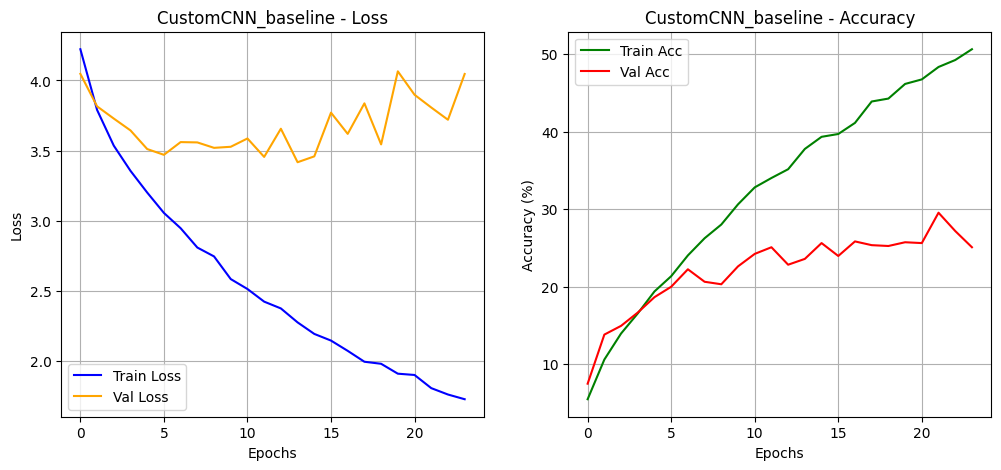
\includegraphics[width=1\textwidth]{images/perf1.png}
    \caption{Training and Validation Performance of Custom CNN.}
    \label{fig:custom_cnn_perf}
\end{figure}
\noindent
The experimental results of the Custom CNN ~\ref{fig:custom_cnn_perf} reveal a sharp divergence between training and validation metrics occurring as early as the fifth epoch. This trend indicates that the network, due to its shallow architecture and the absence of pre-trained weights, quickly exhausts its representational capacity. Instead of learning generalizable action patterns, the model begins to memorize the training data noise, leading to severe overfitting.\\\\
A final test accuracy of 27.76\% provides quantitative evidence that the dataset and the task’s complexity substantially exceed the model’s capacity, making it inadequate for reliable action recognition. In essence, this outcome underlines the necessity of transitioning from a \textit{"proof-of-concept"} scratch-trained model to a more advanced, deeper architecture that leverages the benefits of transfer learning.



\subsection{ResNet18 with temporal mean pooling: Training and results}

\begin{itemize}
    \item \textbf{Fine-tuning Strategy}: Adaptation of ResNet18 to the UCF101 dataset, preserving pre-trained spatial features.
    \item \textbf{Optimization}: Categorical Cross-Entropy loss paired with the Adam optimizer.
    \item \textbf{Learning Rate}: $\eta = 10^{-5}$ for a maximum of 50 epochs, ensuring conservative weight updates.
    \item \textbf{Validation Policies}: Model Checkpointing and Early Stopping with a patience of 10 epochs ($\Delta = 0.001$).
    \item \textbf{Data Pipeline}: Optimized batch size of 32 with data shuffling.
\end{itemize}

\begin{table}[h]
\centering
\caption{Top 5 Worst and Best Performing Classes}
\label{tab:class_accuracy_extremes}
\begin{tabular}{l c @{\quad} l c}
\toprule
\multicolumn{2}{c}{\textbf{Most Difficult Classes}} &
\multicolumn{2}{c}{\textbf{Best Performing Classes}} \\
\cmidrule(r){1-2} \cmidrule(l){3-4}
\textbf{Class Name} & \textbf{Accuracy (\%)} &
\textbf{Class Name} & \textbf{Accuracy (\%)} \\
\midrule
HandstandWalking & 0.00  & SumoWrestling     & 100.00 \\
JumpRope         & 2.63  & Skijet            & 100.00 \\
BodyWeightSquats & 10.00 & Surfing           & 100.00 \\
Nunchucks        & 11.43 & Rafting           & 100.00 \\
WallPushups      & 20.00 & VolleyballSpiking & 100.00 \\
\bottomrule
\end{tabular}
\end{table}

\begin{figure}[h]
    \centering
    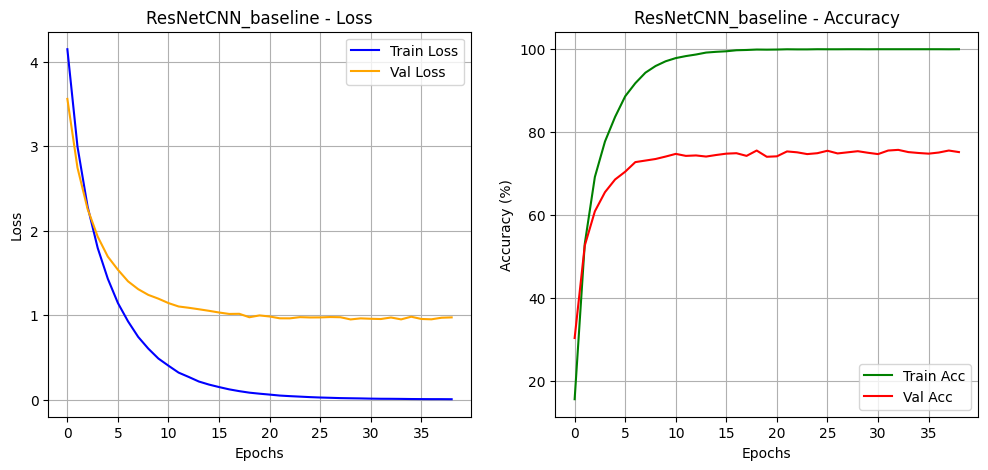
\includegraphics[width=1\textwidth]{images/perf2.png}
    \caption{Training and Validation Performance of ResNet18 with Temporal Mean Pooling.}
    \label{fig:custom_cnn_perf2}
\end{figure}

\noindent
As shown in Figure~\ref{fig:custom_cnn_perf2}, the transition to a ResNet18 backbone yields a 75.71\% test accuracy. However, the model fails on purely dynamic actions such as \textit{HandstandWalking} (0\%) and \textit{JumpRope} (2.63\%) (Table~\ref{tab:class_accuracy_extremes}). Because the \textit{Bag-of-Frames} approach collapses the temporal dimension, the architecture remains a scene classifier unable to distinguish motion-dependent patterns. This "temporal collapse" justifies the transition to a sequential architecture to capture the missing dynamics.




\subsection{ResNet18 with LSTM: Training and results}

The training process for the ResNet-LSTM architecture utilizes several advanced strategies to optimize the end-to-end fine-tuning:

\begin{itemize}
    \item \textbf{Differential Learning Rates}: We employ the \textbf{AdamW} optimizer with a weight decay of $10^{-4}$. To balance feature preservation and temporal adaptation, the backbone uses $\eta = 10^{-5}$, while the LSTM and classifier modules use $\eta = 10^{-4}$.
    \item \textbf{Label Smoothing}: The cross-entropy loss incorporates a \textbf{label smoothing} factor of $0.1$ to improve generalization and prevent the model from becoming overconfident on the complex UCF101 samples.
    \item \textbf{Learning Rate Scheduling}: A \textbf{ReduceLROnPlateau} scheduler is implemented, reducing the learning rate by a factor of $0.1$ if the validation loss plateaus for $7$ consecutive epochs.
    \item \textbf{Convergence Control}: Given the increased complexity of the recurrent module, the early stopping \textbf{patience} is extended to $15$ epochs (with a delta of $0.001$) to allow for stable convergence.
\end{itemize}


\begin{figure}[h]
    \centering
    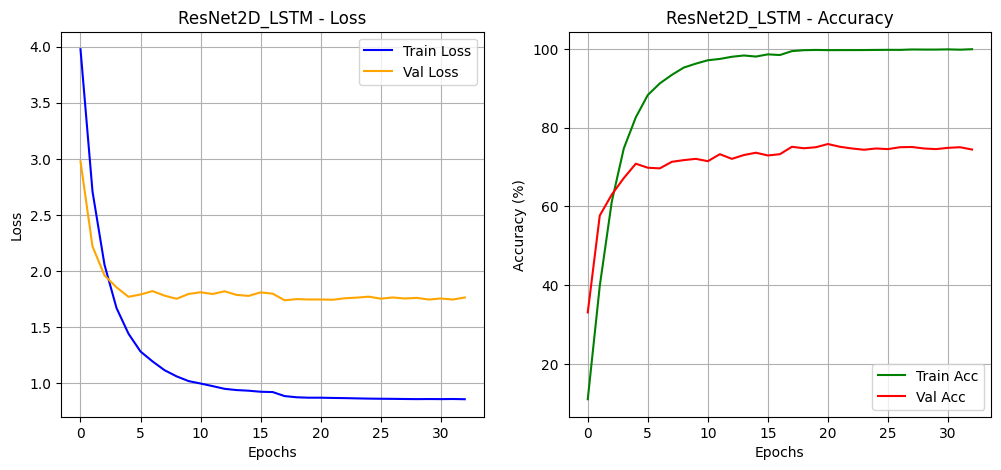
\includegraphics[width=1\textwidth]{images/perf3.png}
    \caption{Training and Validation Performance of ResNet18+LSTM.}
    \label{fig:cnn_perf3}
\end{figure}

\noindent
The results of the training and validation in figure~\ref{fig:cnn_perf3} show that the model has a very high learning capacity, reaching 100\% training accuracy quickly. However, the gap between training and validation loss is wider than in the simple ResNet baseline, suggesting that adding an LSTM makes the model more complex and prone to overfitting.\\\\
The test results shown that the final accuracy is 73.88\%, a slight decrease from the 75.71\% of the previous ResNet-only model. However, the table of class extremes shows a vital improvement in dynamic actions:
\begin{itemize}
    \item \textbf{Action Recognition}: Purely dynamic classes are finally recognized. \textit{HandstandWalking} jumped from 0\% to \textbf{20.59\%}, proving the LSTM is capturing temporal patterns previously ignored.
    \item \textbf{Static Backgrounds}: Top-performing classes remain at \textbf{100\% accuracy}, as the ResNet backbone easily identifies their unique visual environments.
    \item \textbf{Unidirectional Limits}: Classes with fast, repetitive motions like \textit{JumpRope} (5.26\%), \textit{Nunchucks} (11.43\%), \textit{YoYo} (13.89\%) remain difficult.
\end{itemize}

\begin{table}[h]
\centering
\caption{Top 5 Worst and Best Performing Classes with ResNet18+LSTM}
\label{tab:class_accuracy_extremes_updated}
\begin{tabular}{l c @{\quad} l c}
\toprule
\multicolumn{2}{c}{\textbf{Most Difficult Classes}} &
\multicolumn{2}{c}{\textbf{Best Performing Classes}} \\
\cmidrule(r){1-2} \cmidrule(l){3-4}
\textbf{Class Name} & \textbf{Accuracy (\%)} &
\textbf{Class Name} & \textbf{Accuracy (\%)} \\
\midrule
JumpRope          & 5.26  & PlayingFlute  & 100.00 \\
Nunchucks         & 11.43 & Diving        & 100.00 \\
YoYo              & 13.89 & PlayingViolin & 100.00 \\
HandstandWalking  & 20.59 & Rowing        & 100.00 \\
BrushingTeeth     & 27.78 & Surfing       & 100.00 \\
\bottomrule
\end{tabular}
\end{table}


\subsection{ResNet18 with BiLSTM: Training and results}
The ResNet18-BiLSTM architecture represents a significant evolution in our temporal modeling, utilizing a bidirectional approach to capture dependencies from both the past and future states of a sequence. The training strategy is detailed below:

\begin{itemize}
    \item \textbf{Differential Learning Rates}: To ensure stable end-to-end fine-tuning, we employ the \textbf{AdamW} optimizer with a weight decay of $10^{-4}$. We apply a stratified learning rate strategy: the ResNet18 backbone is tuned with $\eta = 10^{-5}$ to preserve pretrained spatial features, while the BiLSTM and the MLP classifier use $\eta = 10^{-4}$.
    \item \textbf{Robust Regularization}: Beyond the standard \textbf{Label Smoothing} ($0.1$), we implement a multi-stage dropout strategy. This includes \textbf{Spatial Dropout} ($0.6$) on the extracted features and specific dropout layers within the BiLSTM ($0.5$) and the final classifier to mitigate overfitting on the UCF101 dataset.
    \item \textbf{Gradient Management}: To prevent gradient explosions common in deep recurrent networks, we apply \textbf{Gradient Clipping} with a maximum norm of $1.0$.
    \item \textbf{Optimization Scheduling}: We utilize the \textbf{ReduceLROnPlateau} scheduler, which monitors the validation loss and reduces the learning rate by a factor of $0.1$ after $7$ epochs of stagnation. The training is governed by an \textbf{Early Stopping} policy with a patience of $15$ epochs to ensure the model reaches its optimal generalization point.
\end{itemize}


\begin{figure}[h]
    \centering
    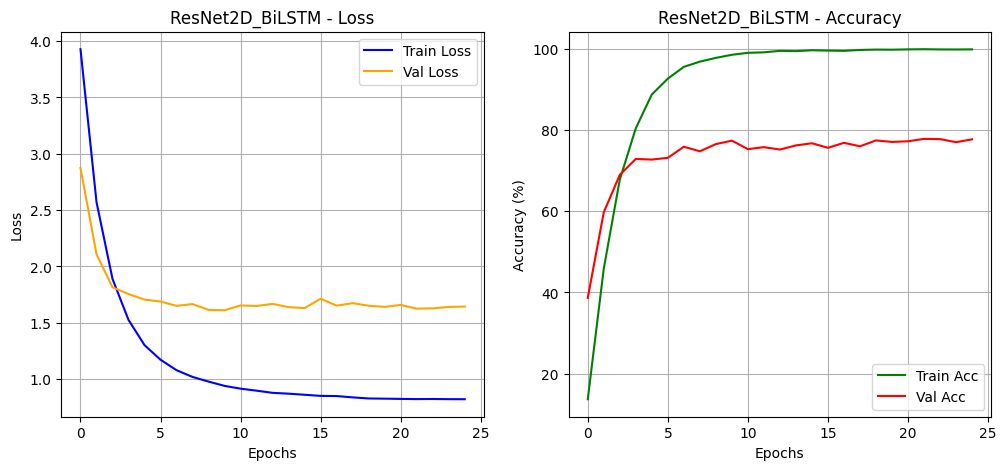
\includegraphics[width=1\textwidth]{images/perf4.png}
    \caption{Training and Validation Performance of ResNet18+BiLSTM.}
    \label{fig:cnn_perf4}
\end{figure}

\noindent
As shown in Figure \ref{fig:cnn_perf4}, the model exhibits rapid convergence, with training accuracy reaching near-saturation within 15 epochs. While a gap between training and validation performance suggests a degree of overfitting, the stability of the validation loss indicates successful regularization through spatial dropout ($0.6$) and weight decay.\\\\
The ResNet18-BiLSTM model achieved a final test accuracy of \textbf{78.14\%}, demonstrating a significant improvement (+7.04\%) over the original RGB-only LRCN baseline of 71.1\%. The results provide deep insights into the model's ability to synthesize temporal information.\\\\
The classification performance reveals a clear distinction between actions:
\begin{itemize}
    \item \textbf{Top Performers}: Classes such as \textit{PlayingPiano}, \textit{Typing}, and \textit{Surfing} achieved \textbf{100\% accuracy}. These categories benefit from strong spatial cues and consistent environmental backgrounds that the ResNet18 backbone identifies with high confidence.
    \item \textbf{Failure Cases and Temporal Gain}: The model lowest scores represent a measurable improvement over previously models. This suggests that the BiLSTM is extracting motion cues that were previously inaccessible. This transition from static scene recognition to dynamic action understanding confirms that the recurrent layers are effectively modeling the chronological evolution of the sequences, even in high-ambiguity scenarios.
\end{itemize}

\begin{table}[h]
\centering
\caption{Top 5 Worst and Best Performing Classes on the Test Set}
\label{tab:final_class_accuracy_extremes}
\begin{tabular}{l c @{\quad} l c}
\toprule
\multicolumn{2}{c}{\textbf{Most Difficult Classes}} &
\multicolumn{2}{c}{\textbf{Best Performing Classes}} \\
\cmidrule(r){1-2} \cmidrule(l){3-4}
\textbf{Class Name} & \textbf{Accuracy (\%)} &
\textbf{Class Name} & \textbf{Accuracy (\%)} \\
\midrule
HandstandWalking & 17.65 & PlayingPiano & 100.00 \\
JumpRope         & 26.32 & Surfing      & 100.00 \\
CricketShot      & 28.57 & Skijet       & 100.00 \\
Nunchucks        & 37.14 & Rowing       & 100.00 \\
BodyWeightSquats & 40.00 & Typing       & 100.00 \\
\bottomrule
\end{tabular}
\end{table}

\subsection{Transformer VideoMAE: Training and Results}

The fine-tuning of the VideoMAE architecture utilizes a high-capacity Transformer backbone, specifically the \texttt{videomae-base} variant, which benefits from extensive self-supervised pre-training on the Kinetics-400 dataset for 1,600 epochs \cite{Tong2022}. To adapt this "Masked Autoencoder" for the supervised classification task on UCF101, we implemented the following protocol:

\begin{itemize}
    \item \textbf{Input Pipeline and Dimensionality}: The model processes clips of 16 frames with a resolution of $224 \times 224$. Unlike convolutional models, we applied a dimension \textbf{permutation} to the input tensor, shifting the temporal dimension before the color channels $(B, T, C, H, W)$ to satisfy the Transformer's attention mechanism requirements.
    \item \textbf{Optimization Strategy}: We utilized the \textbf{AdamW} optimizer with a conservative learning rate of $\eta = 5 \times 10^{-5}$. This choice prevents the massive pre-trained weights from being "washed away" by large gradients during the initial epochs, focusing instead on stabilizing the newly initialized classification head.
    \item \textbf{Loss and Regularization}: To mitigate the high risk of overfitting associated with Vision Transformers (ViT) on medium-sized datasets, we employed \textbf{Cross-Entropy Loss with Label Smoothing} ($0.1$). This encourages the model to be less overconfident, facilitating better generalization during the transfer learning process.
    \item \textbf{Inference Constraints}: To maintain a focus on computational efficiency and real-time applicability, we adopted a \textbf{single-view inference} strategy, processing only the central clip of each video rather than the computationally expensive multi-view approach typically seen in literature \cite{Tong2022}.
\end{itemize}


\begin{figure}[h]
    \centering
    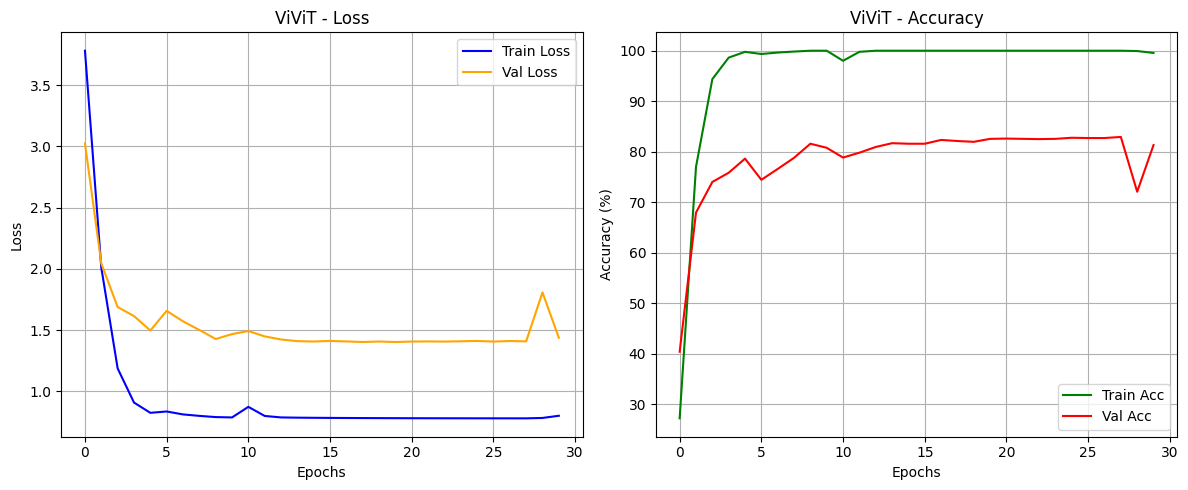
\includegraphics[width=1\textwidth]{images/perf5.png}
    \caption{Training and Validation Performance of fine-tuned VideoMAE-base.}
    \label{fig:cnn_perf5}
\end{figure}

The VideoMAE-base model achieved a peak validation accuracy of \textbf{82.92\%}, establishing itself as the superior architecture in our comparative study. However, the training dynamics reveal a profound "generalization gap" that warrants technical discussion.


\begin{itemize}
    \item \textbf{Rapid Convergence}: The model reached $100\%$ training accuracy by Epoch 9. This suggests that the self-supervised pre-training on Kinetics-400 provided such rich spatiotemporal features that the model effectively "memorized" the UCF101 training distribution almost instantly \cite{Tong2022}.
    \item \textbf{Performance Delta}: Despite the overfitting, VideoMAE outperformed the ResNet18-BiLSTM baseline by $+4.62\%$. This confirms that global self-attention mechanisms are inherently better at capturing the complex dynamics of actions like \textit{CricketShot} or \textit{JumpRope} compared to recurrent hidden states.
    \item \textbf{Saturation and Plateau}: The stagnation of the validation loss around $1.40$ indicates that without advanced data augmentation (e.g., Mixup or RandAugment), the model's high capacity leads to a representational bottleneck where further training only reinforces existing biases rather than discovering new discriminative features \cite{Tong2022}.
\end{itemize}

\subsubsection{Addressing the Gap with State-of-the-Art Benchmarks}
It is important to contextualize our result of $82.92\%$ against the published SOTA of $96.1\%$ for VideoMAE on UCF101 \cite{Tong2022}. This discrepancy is not indicative of architectural failure, but rather of the simplified evaluation protocol adopted for this study:

\begin{enumerate}
    \item \textbf{Inference Protocol}: SOTA benchmarks utilize \textbf{multi-view testing}, typically averaging predictions over 12 views (3 temporal clips $\times$ 4 spatial crops) per video \cite{Tong2022}. Our study employs a single-view, single-crop inference to prioritize real-time feasibility.
    \item \textbf{Data Augmentation}: Official results rely on heavy regularization techniques such as \textit{Mixup}, \textit{CutMix}, and \textit{RandAugment}, which are essential to prevent Transformers from overfitting on smaller datasets like UCF101.
    \item \textbf{Supervised Pre-training}: While our model uses self-supervised weights, SOTA results often start from checkpoints already fine-tuned on the full Kinetics-400 labels, providing a more discriminative starting point.
\end{enumerate}

The final evaluation on the test set yielded an accuracy of \textbf{79.0\%} for the VideoMAE model. While this represents a marginal improvement of \textbf{+1\%} over the ResNet18-BiLSTM baseline (78\%), the results suggest that both architectures encounter a similar performance ceiling when constrained to single-view inference and a 16-frame temporal window. \\
As illustrated in Table \ref{tab:worst5_classes_final}, the classes that pose the greatest challenge remain largely consistent across both modeling paradigms. 

\begin{table}[h]
\centering
\caption{Top 5 Most Difficult Classes on the Test Set}
\label{tab:worst5_classes_final}
\begin{tabular}{l c}
\toprule
\textbf{Class Name} & \textbf{Accuracy (\%)} \\
\midrule
BrushingTeeth     & 11.11 \\
HandstandWalking  & 20.59 \\
Nunchucks         & 22.86 \\
ShavingBeard      & 30.23 \\
Hammering         & 30.30 \\
\bottomrule
\end{tabular}
\end{table}

\noindent
In conclusion, without advanced data augmentation or multi-crop evaluation, the latent representational power of the Transformer cannot fully compensate for the lack of high-frequency spatial details.
\section{Conclusions}

This study provided a systematic exploration of Human Action Recognition (HAR) using the UCF101 benchmark, tracking the evolution of architectural paradigms from spatial feature aggregation to advanced attention-based modeling. The objective was to quantify the performance gains associated with increasingly complex temporal reasoning and to evaluate the feasibility of fine-tuning large-scale Transformers in a single-view, efficient inference setting.

\subsection{Summary of Results}
The experimental results confirm a clear hierarchy of performance aligned with the chronological and technical evolution of computer vision:
\begin{itemize}
    \item \textbf{Baseline Performance}: The spatial-only ResNet-50 approach established a performance floor, demonstrating that environment and object recognition provide a significant but incomplete foundation for action understanding.
    \item \textbf{The Value of Recurrence}: The transition to a bidirectional sequential model (ResNet18-BiLSTM) yielded a test accuracy of \textbf{78.14\%}. This $+7\%$ improvement over standard RGB-only baselines proves that modeling the chronological evolution of movement is essential for distinguishing actions with similar spatial contexts.
    \item \textbf{Transformer Performance}: The \textbf{VideoMAE-base} architecture achieved the highest performance in this study with a validation accuracy of \textbf{82.76\%}. Despite significant overfitting—evidenced by rapid training saturation—the global self-attention mechanism demonstrated superior capacity in capturing long-range spatiotemporal dependencies compared to recurrent hidden states.
\end{itemize}

\subsection{Final Considerations}
The gap between our experimental results ($82.76\%$) and the state-of-the-art benchmarks ($96.1\%$) highlights the critical role of evaluation protocols and regularization. While our study prioritized computational efficiency and single-view feasibility, the literature suggests that peak performance is contingent upon multi-view testing and aggressive data augmentation. Nevertheless, the consistent performance delta across the models validates our incremental methodology and confirms the transition toward attention-based systems as the most effective path for future research.




\printbibliography


\end{document}
